% This LaTeX was auto-generated from MATLAB code.
% To make changes, update the MATLAB code and export to LaTeX again.

\documentclass{article}

\usepackage[utf8]{inputenc}
\usepackage[T1]{fontenc}
\usepackage{lmodern}
\usepackage{graphicx}
\usepackage{color}
\usepackage{hyperref}
\usepackage{amsmath}
\usepackage{amsfonts}
\usepackage{epstopdf}
\usepackage[table]{xcolor}
\usepackage{matlab}

\sloppy
\epstopdfsetup{outdir=./}
\graphicspath{ {./logistic_regression_example_images/} }

\begin{document}

\matlabtitle{Logistic Regression example}

\begin{matlabcode}
rng(5)
X1 = rand([100,1])*2.+1;
X2 = rand([100,1])*3.;
y = double(X2>X1.*1.5-1)
\end{matlabcode}
\begin{matlaboutput}
y = 100x1    
     1
     0
     0
     0
     0
     0
     0
     0
     1
     1

\end{matlaboutput}
\begin{matlabcode}

X = [X1 X2];

f=gscatter(X1,X2,y,'br','o');
hold on
plot(X1,X1.*1.5-1,'g')
legend('0','1','Real separation','Location','northoutside')
hold off
\end{matlabcode}
\begin{center}
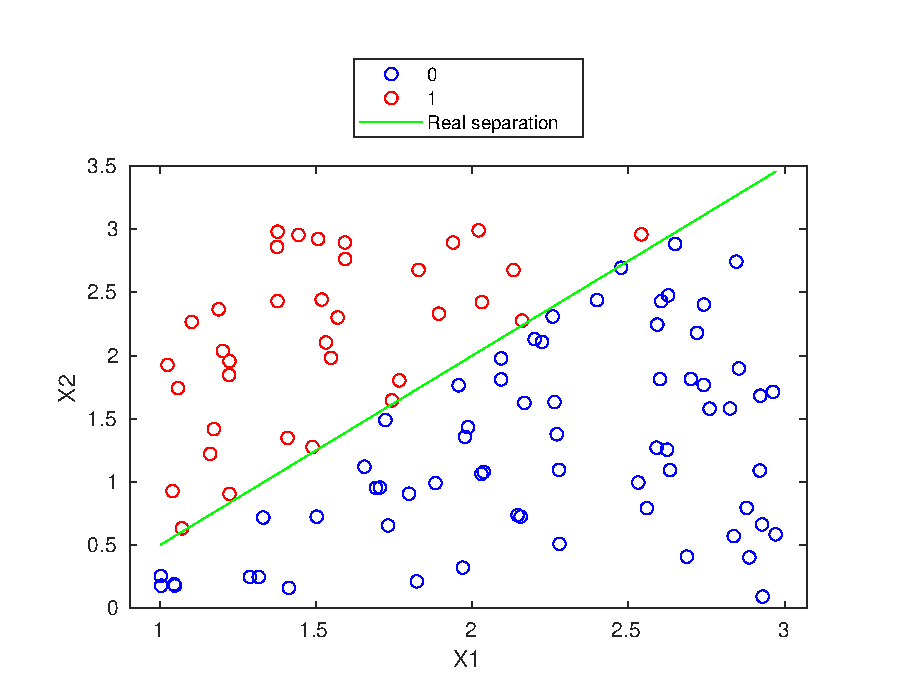
\includegraphics[width=\maxwidth{56.69844455594581em}]{figure_0.eps}
\end{center}


\begin{par}
\begin{flushleft}
Let's train using gradient descent:
\end{flushleft}
\end{par}

\begin{matlabcode}
[n, d] = size(X);
X_bias = [ones(n,1) X]
\end{matlabcode}
\begin{matlaboutput}
X_bias = 100x3    
    1.0000    1.4440    2.9554
    1.0000    2.7415    2.4042
    1.0000    1.4134    0.1619
    1.0000    2.8372    0.5714
    1.0000    1.9768    1.3573
    1.0000    2.2235    2.1088
    1.0000    2.5318    0.9961
    1.0000    2.0368    1.0799
    1.0000    1.5936    2.7644
    1.0000    1.3754    2.8609

\end{matlaboutput}
\begin{matlabcode}

[W,niter] = train_GD(X_bias,y,0.1,1e-3,20)
\end{matlabcode}
\begin{matlaboutput}
W = 3x1    
    3.9647
  -13.2924
   13.2435

niter = 20
\end{matlaboutput}
\begin{matlabcode}

y_hat = my_predict(X_bias,W);

f2=gscatter(X1,X2,y_hat,'br','o');
hold on
plot(X1,X1.*1.5-1,'g')
legend('0','1','Real separation','Location','northoutside')
hold off
\end{matlabcode}
\begin{center}
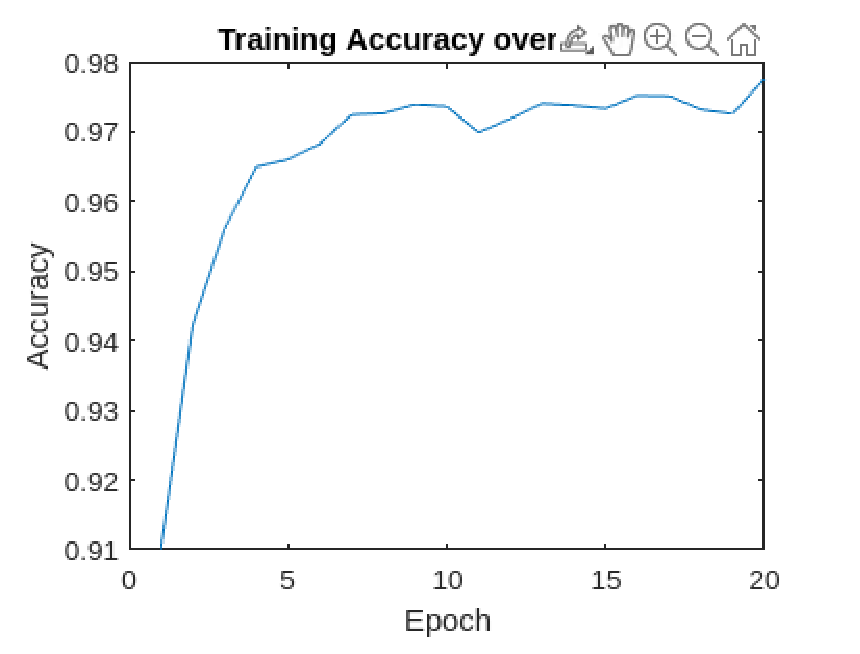
\includegraphics[width=\maxwidth{56.69844455594581em}]{figure_1.eps}
\end{center}

\begin{par}
\begin{flushleft}
We can observe how it is quite ok... Let's increment the max\_iter parameters:
\end{flushleft}
\end{par}

\begin{matlabcode}
[W,niter] = train_GD(X_bias,y,0.1,1e-3,1000)
\end{matlabcode}
\begin{matlaboutput}
W = 3x1    
   20.9642
  -27.7530
   17.3205

niter = 1000
\end{matlaboutput}
\begin{matlabcode}

y_hat = my_predict(X_bias,W);

f3=gscatter(X1,X2,y_hat,'br','o');
hold on
plot(X1,X1.*1.5-1,'g')
legend('0','1','Real separation','Location','northoutside')
hold off
\end{matlabcode}
\begin{center}
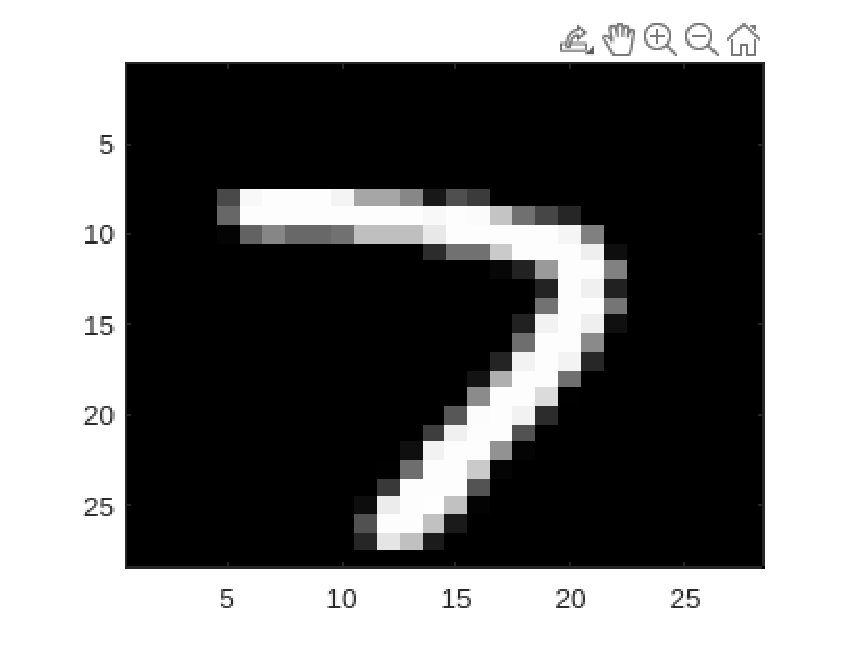
\includegraphics[width=\maxwidth{56.69844455594581em}]{figure_2.eps}
\end{center}

\begin{par}
\begin{flushleft}
And in fact it is much better! :D
\end{flushleft}
\end{par}

\begin{par}
\begin{flushleft}
Let's see how IRLS performs:
\end{flushleft}
\end{par}

\begin{matlabcode}
[W,niter_NR] = train_NR(X_bias,y,1e-3,1000,1e-3)
\end{matlabcode}
\begin{matlaboutput}
W = 3x1    
1.0e+05 *

    1.6554
   -2.0991
    1.2912

niter_NR = 227
\end{matlaboutput}
\begin{matlabcode}

y_hat = my_predict(X_bias,W);

f4=gscatter(X1,X2,y_hat,'br','o');
hold on
plot(X1,X1.*1.5-1,'g')
legend('0','1','Real separation','Location','northoutside')
hold off
\end{matlabcode}
\begin{center}
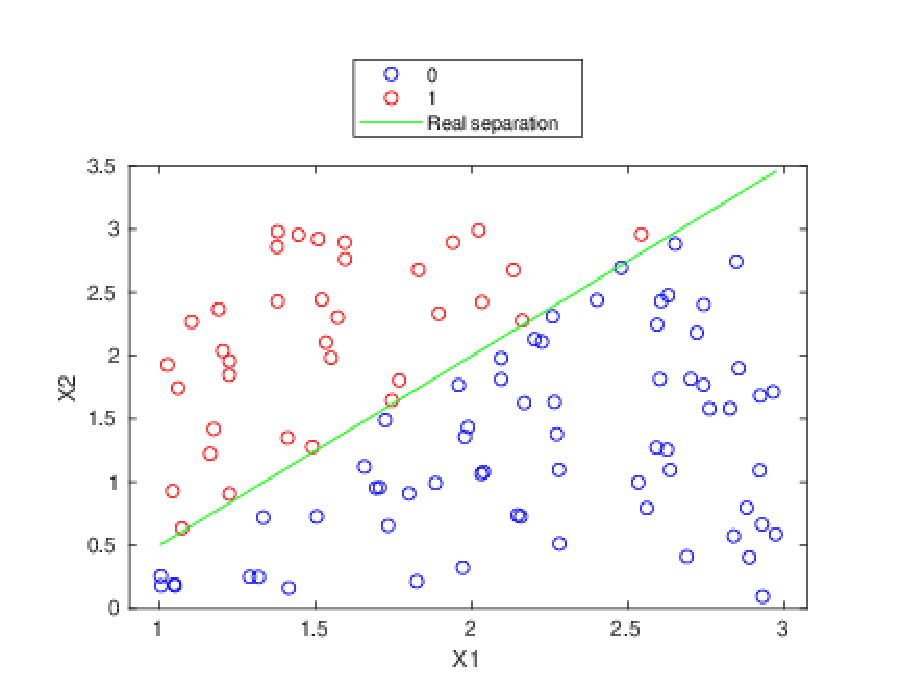
\includegraphics[width=\maxwidth{56.69844455594581em}]{figure_3.eps}
\end{center}

\begin{par}
\begin{flushleft}
We can see how this time we also obtain nice separation, and this one even finishes before maxiter is reached. In fact, we can try to see how many iterations would GD need:
\end{flushleft}
\end{par}


\begin{matlabcode}
[W,niter_GD] = train_GD(X_bias,y,0.1,1e-3,1000000)
\end{matlabcode}
\begin{matlaboutput}
W = 3x1    
  110.2037
 -146.6376
   92.3106

niter_GD = 449262
\end{matlaboutput}

\begin{par}
\begin{flushleft}
Therefore, we obtain an enormous speedup:
\end{flushleft}
\end{par}


\begin{matlabcode}
speedup = niter_GD / niter_NR
\end{matlabcode}
\begin{matlaboutput}
speedup = 1.9791e+03
\end{matlaboutput}

\begin{par}
\begin{flushleft}
Almost 2000 times faster in terms of iterations...
\end{flushleft}
\end{par}


\begin{matlabcode}
function S = state(X, W)
    S = X*W;
end

function s=logistic(S)
    s = 1./(1+exp(-S));
end

function ds=grad_logistic(y, y_hat, X)
    ds = X' * (y_hat - y);
end

function H = hess_logistic(y_hat, X)
    D = diag(y_hat .* (1 - y_hat));
    H = X' * D * X;
end


function [W,niter]=train_GD(X, y, lr, threshold, maxiter)
    [~, d] = size(X);
    W = ones(d, 1);
    for niter=1:maxiter
        st = state(X,W);
        y_hat = logistic(st);
        ds = grad_logistic(y, y_hat, X);
        v = vecnorm(abs(ds));
        if v < threshold
            break
        end
        W = W - lr*ds;
    end
end

function [W, niter] = train_NR(X, y, threshold, maxiter, lambda)
    [~, d] = size(X);
    W = ones(d, 1);
    I = eye(d);
    for niter = 1:maxiter
        st = state(X, W);
        y_hat = logistic(st);
        gradient = grad_logistic(y, y_hat, X);
        v = vecnorm(abs(gradient));
        if v < threshold
            break
        end
        H = hess_logistic(y_hat, X);
        W = W - inv(H + lambda * I) * gradient; %We add a term to avoid singularities
    end
end

function pred = my_predict(X, W)
    p = logistic(state(X, W));
    pred = double(p >= 0.5);
end
\end{matlabcode}

\end{document}
